\documentclass[handout]{beamer}

% !TeX program = lualatex
\usepackage{pacchetti}

%%%%%%%%%%%%%%%%%%%%%%%%%%%%%%%%%%%%%%% COLORI

\definecolor{turquoise}{RGB}{0, 247, 230}
\definecolor{goldenyellow}{RGB}{255, 218, 66}
\definecolor{fuchsia}{RGB}{255, 0, 172}
\definecolor{electric-blue}{RGB}{55, 0, 255}

\definecolor{blond}{RGB}{251,231,161}
\definecolor{skincolor}{RGB}{224,177,132}
\definecolor{idea}{RGB}{254,231,2} 	        %giallo ideee

%%%%%%%%%%%%%%%%%%%%%%%%%%%%%%%%%%%%%%% HEAD COMMANDS	
\newcommand{\inghead}{% 
	\textcolor{darkturquoise}{\LARGE\textbf{Ingredienti}\ }
}

\newcommand{\mathead}{% 
	\textcolor{darkturquoise}{\LARGE\textbf{Materiale utile}\ }
}
\newcommand{\prephead}{% 
	\textcolor{fuchsiapink}{\LARGE\textbf{Preparazione}\ } }
\newcommand{\hinthead}{% 
	\textcolor{cerisepink}{\huge{Tip:}}
}

%%%%%%%%%%%%%%%%%%%%%%%%%%%%%%%%%%%%%% Math commands

% Comandi per i teoremi, definizioni ed esmpi
\theoremstyle{plain}
\newtheorem{thm}{Teorema} % reset theorem numbering for each chapter
\newtheorem{post}{Postulato} % reset theorem numbering for each chapter
\newtheorem{lem}{Lemma}

\theoremstyle{definition}
\newtheorem{defn}{Definizione} % definition numbers are dependent on theorem numbers
\newtheorem{exmp}{Esempio} % same for example numbers
\newtheorem*{ach}{Attenzione!}

% Shortcut
\newcommand{\SigmaX}{\hat{\sigma}^{(x)}}
\newcommand{\SigmaY}{\hat{\sigma}^{(y)}}
\newcommand{\SigmaZ}{\hat{\sigma}^{(z)}}

\newcommand{\Hilb}{\mathcal{H}}
\newcommand{\Id}{\hat{\mathcal{I}}}
\newcommand{\LinSet}{\mathscr{L}}
\newcommand{\ChoiState}[1]{\hat{\rho}_\text{CJ}^{#1}}

\DeclareMathOperator{\Tr}{tr}

\newcommand{\VerticalBrace}[4][]{%
	% #1 = draw options
	% #2 = top mark
	% #2 = bottom mark
	% #4 = label
	\begin{tikzpicture}[overlay,remember picture]
	\tikzmath{coordinate \p,\q;\p=(pic cs:#2);\q=(pic cs:#3);\maxx=max(\px,\qx);}
	\draw[xshift=1ex,decorate,decoration={brace, amplitude=1.5ex}, #1] 
	([yshift=1.5ex]{{pic cs:#2} -| \maxx pt,0})  -- ([yshift=-.5ex]{{pic cs:#3} -| \maxx pt,0})
	node[My Node Style] {#4};
	\end{tikzpicture}
}


%box carini
\newenvironment<>{ideablock}[1]{%
	\setbeamercolor{block title}{fg=white,bg=fuchsia}%
	\begin{block}#2{#1}}{\end{block}}

\newenvironment<>{defblock}[1]{%
	\setbeamercolor{block title}{fg=white,bg=goldenyellow}%
	\begin{block}#2{#1}}{\end{block}}

\newenvironment<>{theoblock}[1]{%
	\setbeamercolor{block title}{fg=white,bg=turquoise!80!black}%
	\begin{block}#2{#1}}{\end{block}}


% due nuovi comandi per allineare le cose bene
\newcommand\parallelcontent[2]{
	\begin{columns}[t]
		\column{0.5\textwidth} #1
		\column{0.5\textwidth} #2
	\end{columns}
}
\newcommand\parallelitem[2]{
	\parallelcontent
	{\begin{itemize} \item #1 \end{itemize}}
	{\begin{itemize} \item #2 \end{itemize}}
}

%Citazioni
\newcommand{\easycite}[2]{
	[\textcolor{electric-blue}{#1 - #2}]
}

%%%%%%%%%%%%%%%%%%%%%%%%%%%%%%%%%%%%%%% MATH SYMBOLS
\newcommand{\R}{{\mathbb{R}}}
\newcommand{\N}{{\mathbb{N}}}

 \newcommand{\pprec}{\prec\mathrel{\mkern-5mu}\prec}

% % Bibliografia
% \usepackage[backend=bibtex,doi=false,isbn=false,url=false]{biblatex}
% \addbibresource{bibliografia.bib}

\usetheme{PaloAlto}
\setbeamercovered{transparent} %per rendere sbiadito cio' che verra'
\setbeamertemplate{navigation symbols}{}

\usecolortheme{rose} 
\setbeamercolor{structure}{fg=turquoise!70!black}


%Information to be included in the title page:
\title[Generalization of BH Area theorem]
{A generalization of the Black Holes Area Theorem}

\author[Veronica Sacchi]{Veronica Sacchi}      
\institute[SNS]{
\includegraphics[height=1.45cm]{Immagini/logoSNS/orizzontale-colore/orizzontale-colore.pdf}}
\date[16-06-2022]{16th June 2022}
%\logo{
\includegraphics[height=1.1cm]{Immagini/logoSNS/tondo-colore/tondo-colore.png}}

\begin{document}	
	
%	\usebackgroundtemplate{
%		\adjustbox{height=0.8\paperheight, raise=-9cm, right=15cm}{
%			\transparent{0.05}
%			
\includegraphics{Immagini/logoSNS/solo_logo.jpeg}
%		}
%	}
	
	\begin{frame}
	\titlepage
	\end{frame}
	
	\section{Introduction}
	\begin{frame}
		\frametitle{What will we see?}
		\tableofcontents
	\end{frame}

	\subsection{The Classical Black Hole Area Theorem}
	\begin{frame}
		\frametitle{The Classical Black Hole Area Theorem}
		\begin{columns}
			\column{0.33\textwidth}
			\begin{tikzpicture}
			\node[graduate, minimum size = 2.5cm] (A) at (0,0){};
			\node[ellipse callout, draw, yshift= 1.4cm,
					callout absolute pointer={(A.mouth)},
					font=\tiny] {The area of the Black Hole Horizon cannot decrease.};
			\end{tikzpicture}
			\column{0.33\textwidth}
			\column{0.33\textwidth}
		\end{columns}
		
	\end{frame}

	\section{Averaged Energy Conditions}
	\begin{frame}
		\frametitle{Energy Conditions}
		\begin{defblock}{What is an energy condition?}
			It is a condition on a contraction of the stress energy tensor.

			E.g. the Null Energy condition (NEC) is written as \(T_{\mu\nu}k^{\mu}k^{\nu} \ge 0\) for any null vector \(k\).
		\end{defblock}
		\begin{itemize}
			\item Via Einstein equations thay can be translated into a condition on the Ricci tensor.
			\item They aim to express ``attractiveness of gravity", or in general should be related to the ``stability of the system".
		\end{itemize}
		\vskip 10 pt 
		\begin{center}
			\textbf{BUT}
		\end{center}
		\begin{ideablock}{}
			\centering
			All \emph{pointwise} energy conditions will be violated by quantum fields.% \easycite{Epstein, Glaver, Jaffe}{1965}.
		\end{ideablock}
	\end{frame}

	\begin{frame}
		\frametitle{Averaged Energy Conditions}
		\begin{ideablock}{Quantum intrest}
			\centering
			Local violations are often compensated for, or even overcompensated for, in other regions of spacetime.
		\end{ideablock}
		\[
			\Big\Downarrow
		\]
		\emoji{light-bulb}  Let's average them over a suitable region of spacetime! \emoji{light-bulb} 
		\begin{defblock}{ANEC}
			\[
				\int_{\gamma} T_{\mu\nu}U^{\mu}U^{\nu} d\lambda \ge 0 \dashrightarrow \int_{\gamma}  R_{\mu\nu}U^{\mu}U^{\nu} d\lambda \ge 0
			\]
		\end{defblock}
		\textbf{Problems}
		\begin{itemize}
			\item Often either too weak to prove a singularity theorem, or too strong to be proven by QFT.
			\item No clear physical interpretation.
		\end{itemize}
	\end{frame}

	\section{Index form methods}
	\subsection{Focal Points}
	\begin{frame}
		\frametitle{Focal Points}
		\begin{defblock}{Focal Points}
			Let \(\gamma\) be a geodesic of \(M\) normal to the submanifold \(P\). Then \(\gamma(r)\), where \(r \neq 0\), is a \emph{focal point} of \(P\) along \(\gamma\) provided there is a nonzero \(P\)-Jacobi field \(V\) on \(\gamma\), such that \(V(r) = 0\).
		\end{defblock}
		\vskip 10 pt
		\begin{columns}
			\column{0.6\textwidth}
			A focal point is an \emph{almost}-meeting point of nearby \(P\)-normal geodesics \underline{of the same causal character} of \(\gamma\).
			\column{0.4\textwidth}
			\centering
			\includegraphics[scale=0.5]{example-image-duck}
		\end{columns}

		\begin{ideablock}{Why are they important?}
			\centering
			Past a focal point a geodesic is not ``lenght''-extremizing anymore!
		\end{ideablock}
	\end{frame}

	\begin{frame}
		\frametitle{Index form methods}
		For null geodesics we study the \emph{energy} or \emph{action} functional:
		\[
			E[\gamma] \coloneqq \frac{1}{2}\int_{0}^{l} g(\gamma'(\lambda), \gamma'(\lambda))d\lambda	
		\]
		\begin{ideablock}{``Lenght'' Extremization}
			\centering
			No focal points \(\implies \textbf{H}(V) \equiv\frac{d^2E[\gamma_s]}{ds^2}\Big\vert_{s = 0} < 0\)
		\end{ideablock}
	
		\begin{theoblock}{Existence criteria for focal points}
			If there exists \(f(\lambda)\) such that \(f(0) = 1\), \(f(\ell) = 0\) and
			\[
				\int_{0}^{\ell} \big((n -2)(\nabla_Uf)^2 - f^2R_{\mu\nu}U^{\mu}U^{\nu} \big)(\lambda) d\lambda\le -(n-2)U_{\mu}\mathrm{H}^{\mu}\Big\vert_{\lambda = 0}	
			\]
			then \(\gamma\) contains a focal point to \(P\) before \(\ell\)
		\end{theoblock}
	\end{frame}

	\subsection{The Raychaudhuri's equation}
	\begin{frame}
		\frametitle{The Raychaudhuri's equation}
		\begin{defblock}{The expansion}
			\(\theta\) is the variation of the tranversial area of a congruence of geodesics.
			\[
			\theta = \nabla_{\mu}U^{\mu}	
			\]
		\end{defblock}
		\vskip 10pt
		\begin{columns}
			\column{0.2\textwidth}
			\centering
				\includegraphics[scale=0.3]{example-image-duck}
			\column{0.8\textwidth}
			\begin{align*}
				\frac{D}{D\lambda}\theta &= -\frac{\theta^2}{d - 2} - \sigma_{\mu\nu}\sigma^{\mu\nu} + \omega_{\mu\nu}\omega^{\mu\nu}  - R_{\mu\nu}U^{\mu}U^{\nu} \\
				&\le -\frac{\theta^2}{d - 2} - R_{\mu\nu}U^{\mu}U^{\nu}
			\end{align*}
		\end{columns}
		\vskip 10pt
		\begin{ideablock}{Existence criteria for focal points}
			\centering
			\(\vert\theta\vert \rightarrow +\infty \implies \) 
			a focal point is developed.
		\end{ideablock}
	\end{frame}

	\section{The Black Hole Area Theorem}
	\subsection{The classical proof}
	\begin{frame}
		\frametitle{The Classical Black Hole Area Theorem}

		\begin{columns}
			\column{0.6\textwidth}
			\begin{itemize}
				\item \emph{Causal black hole region} \(B\): \(B \coloneqq M \setminus J^-(\mathscr{I}^+)\).
				\item \emph{Causal event horizion} \(H\): \(H\coloneqq \partial J^-(\mathscr{I}^+) \cap M \).
			\end{itemize}
		
			\column{0.4\textwidth}
			\includegraphics[scale=0.4]{example-image-duck}
		\end{columns}
		\begin{theoblock}{Hawking's Area Theorem}
			Let \((M, g_{\mu\nu})\) be a strongly asymptotically predictable spacetime satisfying \(R_{\mu\nu}k^{\mu}k^{\nu} \ge 0\) for all null vectors \(k^{\mu}\). 
			
			Let \(\Sigma_1\) and \(\Sigma_2\) be spacelike Cauchy surfaces for the globally hyperbolic region \(\tilde{V}\) such that \(\Sigma_2 \subset I^+(\Sigma_1)\), and given \(H\) the event horizon we define
			\[
			\mathscr{H}_1 = H \cap \Sigma_1 \quad \quad \mathscr{H}_2 = H \cap \Sigma_2
			\]
			Then the area of \(\mathscr{H}_2\) is greater or equal than the area of \(\mathscr{H}_1\).
		\end{theoblock}
	\end{frame}

	\begin{frame}{A new proof of the Black Hole Area Theorem}
		\begin{columns}
			\column{0.3\textwidth}
			\includegraphics[scale=0.4]{example-image-duck}
			\column{0.7\textwidth}
			The proof is made of \(2\) main steps
			\begin{enumerate}
				\item Observe that on any Cauchy hypersurface for the null generators of the horizion it holds that \(\mathrm{H}^{\mu}U_{\mu} \ge 0\).
				\item Prove that the above implies the thesis.
			\end{enumerate}
		\end{columns}
		\vskip 7pt
		\textbf{Step \(1\)}: By contradiction \(\exists p\in \mathscr{H}_1\) such that \(\mathrm{H}^{\mu}U_{\mu} < 0\).
		\vskip 7pt
		\begin{columns}
			\column{0.6\textwidth}
			For continuity there exists an outward deformation of \(\mathscr{H}_1\) such that \(\mathrm{H}'^{\mu}U'_{\mu} < 0\) everywhere.

			From NEC and picking \(f(\lambda) = 1 - \frac{\lambda}{\ell}\)
			\column{0.4\textwidth}
			\includegraphics[scale=0.4]{example-image-duck}
		\end{columns}
		\vskip 7pt
		\[
		J_{\ell}[f] \coloneqq \int_{0}^{\ell} \big((n -2)(\nabla_Uf)^2 - f^2R_{\mu\nu}U^{\mu}U^{\nu} \big)(\lambda) d\lambda \le \frac{n - 2}{\ell}
		\]

	\end{frame}

	\begin{frame}[fragile]
		\begin{columns}
			\column{0.27\textwidth}
			\(\quad\) Choose \(\ell \ge \frac{1}{\vert \mathrm{H}'^{\mu}U'_{\mu} \vert} \implies\)
			\column{0.3\textwidth}
			\centering
			The null generator through \(p'\) contains a focal point.
			\column{0.1\textwidth}
			\centering
			\hspace*{-2.5cm}%
			\begin{tikzpicture}
				\usetikzlibrary{decorations.pathmorphing, patterns,shapes}
				\pgfdeclarepatternformonly{zigzag}{\pgfpointorigin}{
					\pgfpoint{2cm}{2cm}}{\pgfpoint{0.35cm}{0.15cm}}{
					\tikz\draw[decoration = {zigzag,segment length = 0.35cm, amplitude = 0.9mm},decorate, thick] (0,1.5) -- (2.9,1.5);
					}
					\begin{scope}[shift={(-5,0)}]
						\draw[decoration = {zigzag,segment length = 3mm, amplitude = 1mm},decorate, color=fuchsia, ultra thick] (0,0)--(0,2.7);
					\end{scope}
			\end{tikzpicture}
			\column{0.33\textwidth}
			\centering
			\underline{Global Hyperbolicity}:
			null generators cannot contain any focal point.
		\end{columns}
		\vskip 10pt
		\textbf{Step \(2\)}:
		\begin{columns}
			\column{0.5\textwidth}
			\begin{itemize}
				\item The image of \(\mathscr{H}_1\) along the flow of null generators is contained in \(\mathscr{H}_2\).
				\item \(\mathrm{H}^{\mu}U_{\mu} \ge 0 \implies \delta_U\mathcal{A}_{\mathscr{H}_1} = \int_{\mathscr{H}_1} \mathrm{H}^{\mu}(p)U_{\mu} \ge 0\).
			\end{itemize}
			\column{0.5\textwidth}
			\centering
			\includegraphics[scale=0.5]{example-image-duck}
		\end{columns}
		
	\end{frame}

	\subsection{A step towards a generalization}
	\begin{frame}
		\frametitle{A step towards a generalization}
		\[
		J_{\ell}[f] \coloneqq \int_{0}^{\ell} \big((n -2)(\nabla_Uf)^2 - f^2R_{\mu\nu}U^{\mu}U^{\nu} \big)(\lambda) d\lambda.
		\]
		\begin{ideablock}{Key observation}
			As soon as we can place an upper bound on \(J_{\ell}[f]\), we obtain a lower bound on \(\mathrm{H}^{\mu}(p)U_{\mu}\).
			\[
				\exists f \quad\vert\quad  J_{\ell}[f] \le (n - 2)\mathcal{V} \implies \mathrm{H}^{\mu}U_{\mu}(p) \ge -\mathcal{V}.
			\]
		\end{ideablock}
		Different energy conditions will provide with different bound on \(J[f]\). The idea is to search for conditions that give a positive bound \(\mathcal{V} \ge 0\).
		\begin{defblock}{Classical conditions}
			Classical energy conditions \(\implies J[f] \le 0\). 
		\end{defblock}

	\end{frame}

	\subsection{The Sobolev condition}
	\begin{frame}
		\frametitle{The Sobolev condition}
		\begin{defblock}{Sobolev condition}
		The Sobolev condition is satisfied on \(\gamma\), for a lenght \(\ell\) if there exist \(m\in\N\) and \(2\) constants \(Q_0\) and \(Q_m\) such that:
		\[
		\forall f \quad
		\int_0^{\ell} f(\lambda)^2 R_{\mu\nu}U^{\mu}U^{\nu} \ge -Q_m(\gamma) \vert\vert f^{(m)}\vert\vert^2 - Q_0(\gamma) \vert\vert f\vert\vert^2;
		\]
		\end{defblock}
		With an additional hypothesis this condition gives an interesting bound on \(J\).
		\[
		\begin{cases}
			\text{Sobolev condition for optimal }\ell \\
			R_{\mu\nu}U^{\mu}U^{\nu}(\lambda) \ge \rho_0 \quad \forall\lambda\in[0,\ell_0]
		\end{cases}	
		\implies
		J[f] \le (n - 2)\mathcal{V}(\ell_0)
		\]
		where
		\[
			(n - 2)\mathcal{V}(\ell_0) = (A_m - 1)\rho_0\ell_0 + \frac{Q_mC_m}{\ell_0} + 2\sqrt{(n - 2)Q_0A_mB_m} > 0
		\]
	\end{frame}

	\subsection{Comparison with the evaporation rate}
	\begin{frame}
		\frametitle{Recover \(T\) dependance}
		To compare \(\mathcal{V}\) with the evaporation of Black Holes we need to estimate \(Q_0\), \(Q_m\), \(\rho_0\) and \(\ell_0\).
		\begin{itemize}
			\item In \(n = 2\) and \(m = 1\) \(Q_0\) and \(Q_1\) can be esitimated by the average over KMS states for non-minimally coupled scalar fields.
			\[
			Q_0 = \frac{32\pi^6}{405}\xi^3 \frac{k_B^2}{\hbar^2}\frac{T^8}{T_{Pl}^6} \quad \quad
			Q_1 = \frac{4\pi\sqrt{\pi}}{3}\xi \left(\frac{T}{T_{Pl}}\right)^2
			\]
			\item From numerical and semi-analytical computations:
			\[
			\rho_0 \simeq -2.7 \cdot 10^{-7} \frac{8\pi k_B}{\hbar^3} T^4	
			\]
		\end{itemize}
	\end{frame}

	\begin{frame}
		\frametitle{Recover \(T\) dependance}
		For \(\ell_0\) we have more options:
		\begin{itemize}
			\item Pick a constant \(\ell_0\); this leads to a bound of the form:
			\[
			\mathcal{V}(\ell_0) = \frac{A_1}{\ell_0}T^2 + (B_1\ell_0 + B_2)T^4 + \ldots
			\]
			\item We can minimize \(\mathcal{V}\) for \(\ell \ge 0\); the minimum is obtained for \(\tilde{\ell}_0 = \sqrt{\frac{3Q_1}{2\vert\rho_0\vert}} \propto \frac{1}{T}\). In this case we find:
			\[
			\mathcal{V}	= \frac{5}{6}\sqrt{\frac{3}{2}Q_1\vert\rho_0\vert} = (8\pi)^2A \cdot \frac{G}{\hbar^2} k_B^3 T^3. 
			\]
		\end{itemize}
	\end{frame}

	\begin{frame}
		\frametitle{Comparison with the evaporation rate}
		\begin{theoblock}{Black Hole Evaporation Rate}
			The rate of evaporation for a Black Hole of mass \(M\) is given by:
			\[
			R_{ev} = \frac{1}{M}\frac{dM}{dT} = (8\pi)^3\beta \frac{G}{\hbar^2} k_B^3T^3 \quad \frac{T}{T_{Pl}} \ll 1
			\]
		\end{theoblock}
		
		
		\begin{columns}
			\column{0.33\textwidth}
			\begin{ideablock}{}
				For the optimal \(\ell_0\) we recover the same \(T^3\) dependance!
			\end{ideablock}
			

			For \(\xi \gtrsim O(10^{-4})\) it holds \(\mathcal{V} \ge R_{ev}\).
			\column{0.67\textwidth}
			\centering
			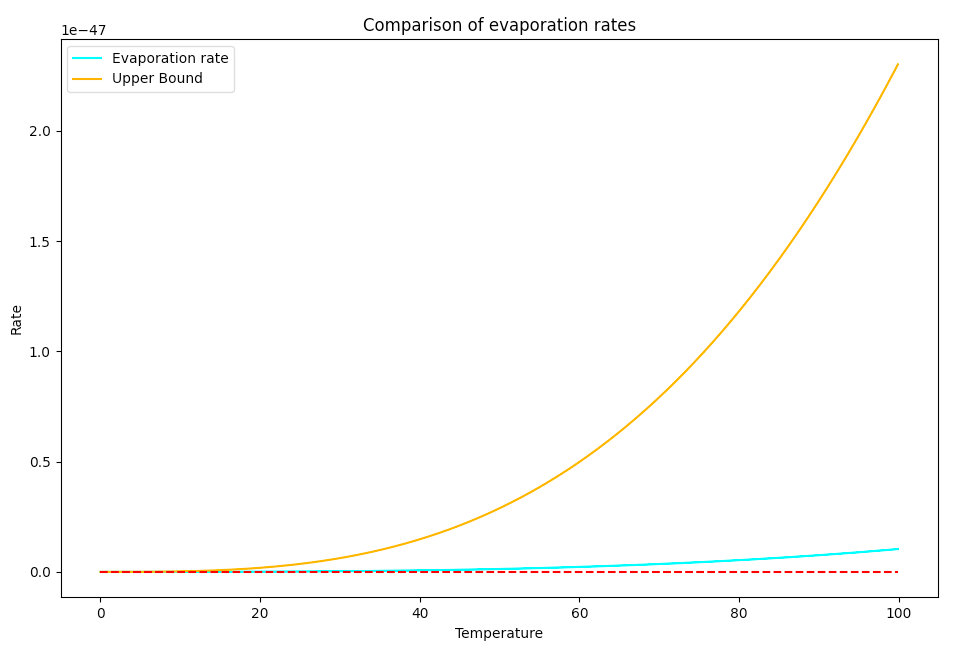
\includegraphics[scale=0.2]{Immagini/ev-rate-conformal.png}
		\end{columns}

	\end{frame}

	
	\section{Further developments}
	\begin{frame}
		\frametitle{What we would like to do next}
		\begin{enumerate}

			\item Look for consistency of the \(T^3\) scaling law of the bound. 
				\begin{itemize}
					\item Average on more states other than the KMS, such as the Unruh state.
					\item Use different functions to place bounds on \(J[f]\).
					\item Assume SNEC instead of Sobolev condition.
				\end{itemize}
			\item  Attempt to place bounds on \(J[f]\) with other different approaches.
			\item Explore what consequences this law will have on black hole thermodynamics.
		\end{enumerate}

		\vskip 22pt

		{\Huge
		\textcolor{turquoise!80!black}{Thank you for your attention!}}
	\end{frame}

\end{document}


	
	
	
	
	
	

	
	
	
	
	



